\chapter{Badania}
\label{cha:badania}
Po przygotowaniu implementacji opisanej w~poprzednim rozdziale przeprowadzona została ewaluacja rozwiązania, w~ramach której badane osoby mogły wypróbować stworzoną grę w~obu przygotowanych wersjach. Badania odbywały się przy pomocy komputera Lenovo Z-50-70 z~zainstalowanym systemem Windows 10. Cechował się następującą konfiguracją sprzętową:
\begin{itemize}
	\item Procesor Intel Core i7-4510U
	\item Karta graficzna NVIDIA GeForce 840M
	\item Pamięć RAM 16GB, DDR3
	\item Rozdzielczość ekranu 1920x1080
\end{itemize}
\section{Procedura eksperymentu}
\begin{enumerate}
	\item Przedstawienie osobie badanej jak będzie wyglądać test. Wspomniano tutaj o~zagraniu przez osobę badaną w~dwie wersje gry. Omówiono także, jak będzie wyglądał montaż urządzeń w~przypadku drugiej wersji gry. 
	\item Przedstawienie sterowania w~pierwszej części gry.
	\item Odpowiedzenie na ewentualne pytania osoby badanej.
	\item Uruchomienie aplikacji w~pierwszej wersji gry.
	\item Pilnowanie czasu gry, wynoszącego od 5~do 10~minut.
	\item Umożliwienie ewentualnej przerwy.
	\item Pomoc osobie badanej w~założeniu opaski do pomiaru tętna i~elektrod na przedramieniu.
	\item Upewnienie się, czy gra poprawnie wykrywa urządzenia. W~razie problemów z~połączeniem ponawiano próbę.
	\item Uruchomienie aplikacji w~wersji afektywnej.
	\item Pilnowanie czasu gry, wynoszącego od 5~do 10~minut.
	\item Wręczenie ankiety osobie badanej.
	\item Odpowiedź na ewentualne pytania osoby badanej, zebranie dodatkowych uwag.
\end{enumerate}
\section{Uczestnicy}
Badania zostały przeprowadzone na 7~osobach, gdzie tylko jedna osoba to kobieta. Wiek osób wahał się od 20~do 30~lat. Większość osób należała do grupy studentów, w~przypadku dwóch były to osoby pracujące w~branży programistycznej. Jedna z~osób charakteryzowała się chorowaniem na nadciśnienie tętnicze, co mogło wpłynąć znacznie na jej wyniki badań i~odczytywanych emocji.
%Opis uczestników, wiek, płeć, ewentualny stan zdrowotny
\section{Analiza wyników}
%Jakie emocje były odczuwane i~jak często, czy uczestnicy byli zainteresowani interfejsem, działaniem samej gry, czy zauważali mechaniki w~zależności od odczuwanych emocji
W ramach badań od uczestników zostały zebrane logi zawierające poziomy \textit{valence} i~\textit{arousal} zwrócone przez przygotowany interfejs do rozpoznawania emocji z~uwzględnieniem odczytów z~akcelerometru. Jako dodatkowy atrybut przydatny do analizy zostały zapisane również wartości cech, dla których dana klasa emocji została określona. Dzięki temu zebrane dane mogą zostać wykorzystane jako uzupełnienie zbioru uczącego użytego do stworzenia modelu rozpoznawania emocji opisanego w~rozdziale~\ref{cha:predykcja}. Innym zdarzeniem zapisanym w~ramach logów były momenty wykrycia napięcia mięśni przez określony w~grze czas. Każdy z~uczestników po przeprowadzeniu badań wypełnił także kwestionariusz zawierający pytania na temat wygody użytkowania stanowiska pomiarowego, satysfakcji z~zaimplementowanych mechanik afektywnych oraz opinii na temat gry. Wszystkie pytania znajdujące się w~kwestionariuszu można znaleźć w~dodatku~\ref{cha:questionary_questions}.

W trakcie wykonywania eksperymentów nie zauważono większych problemów z~podłączeniem urządzeń do aplikacji. W~przypadku sześciu osób eksperyment przebiegł w~pełni poprawnie i~nie wymagały one powtórzenia. W~przypadku jednej osoby napotkano problem w~trakcie rozgrywki polegający na użyciu mocy specjalnej w~przypadku gdy badana osoba nie napinała mięśni przedramienia. Po dokładnym wglądzie okazało się, że w~trakcie badania nastąpiło odklejenie się elektrody referencyjnej, przez co sygnał zwracany przez elektromiograf zawierał dużą ilość szumów, które wpływały na wyliczany w~trakcie rozgrywki średni odczyt. Zwrócono na to uwagę podczas późniejszej analizy logów i~zauważono, że w~dwóch przypadkach wykrycie napięcia mięśni trwało przez dłuższy czas, co jednak nie wpłynęło na samą rozgrywkę, dlatego nie podjęto się powtórzenia badań. Rozkład ilości wykryć napięcia mięśni przedramienia przez osoby badane zostały przedstawione na rysunku~\ref{fig:emg_count}.

\begin{figure}
	\centering
	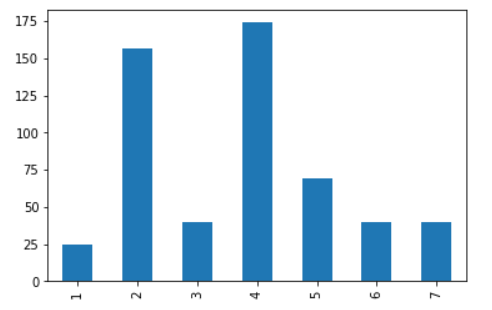
\includegraphics[width=0.6\linewidth]{images/emg_count.png}
	\caption{Ilość wykryć napięcia mięśni przedramienia dla każdej z~badanych osób}
	\label{fig:emg_count}
\end{figure}

W ramach analizy zebranych logów wydzielono zdarzenia zawierające odczyty emocji. Rysunek~\ref{fig:classes_distribution} przedstawia liczebność klas dla wszystkich zebranych pomiarów. Warto zauważyć, że najczęściej występującymi klasami są te, które interpretowane są kolejno jako zrelaksowanie, emocja neutralna oraz smutek. Pierwsze dwie emocje łatwo można wytłumaczyć, ponieważ w~trakcie rozgrywki gracze na początku nie znali jej wszystkich mechanik, natomiast po jakimś czasie od gry przyzwyczaili się do nich i~czerpali z~gry przyjemność. Dziwne wydaje się jednak tak częste występowanie smutku u graczy. Emocja ta wprawdzie mogła się pojawić podczas poznawania mechanik utrudniających rozgrywkę, jednak bardziej adekwatnymi emocjami mogłyby być tutaj złość lub strach. Powodem takiego odczytu mógł być także mechanizm odpowiadający za weryfikację emocji zwróconych przez model uczenia maszynowego przy pomocy odczytów z~akcelerometru. W~przypadku gdy gracz będzie okazywał emocje wyłącznie poprzez zmiany sygnałów fizjologicznych, natomiast kontroler będzie się starał trzymać nieruchomo, wartość \textit{arousal} zostanie zmniejszona. Jeżeli emocją zwróconą przez model w~tym przypadku będzie złość, która jest jedną z~oczekiwanych reakcji na utrudnienie gry, to interfejs po weryfikacji zinterpretuję odczytaną emocję jako smutek.
\begin{figure}[h]
	\centering
	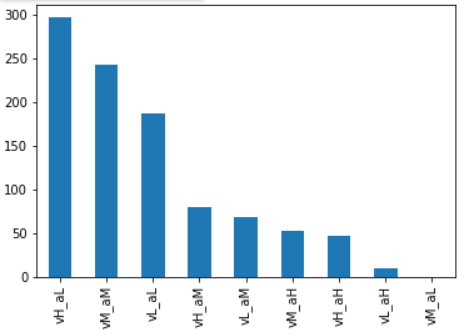
\includegraphics[width=0.6\linewidth]{images/emotions_distribution.png}
	\caption{Liczebność poszczególnych klas zwróconych przez interfejs do rozpoznawania emocji}
	\label{fig:classes_distribution}
\end{figure}

Badani poproszeni o~ocenę trudności gry (tab.~\ref{tab:game_difficulty}), w~przypadku wersji bez pętli afektywnej zgodnie określili ją jako rozgrywkę o~średniej trudności. Co jest ciekawe, w~przypadku wersji afektywnej trzy osoby określiły grę jako trudną, pozostali badani natomiast zostali przy takiej samej ocenie jak w~wersji podstawowej. Podczas odpowiadania na pytania badanych, zauważyli oni, że w~przypadku gry z~pętlą afektywną pojawiało się znacznie więcej mechanik utrudniających grę i~właśnie to mogło prowadzić do takiej oceny. W~przypadku osób, które nie zauważyły różnicy w~trudności, może to sugerować, że wprowadzenie pętli afektywnej nie wpłynęło znacząco na trudność rozgrywki. 
\begin{table}[]
	\centering
	\caption{Ocenienie poziomu trudności gry w~obu jej wersjach}
	\label{tab:game_difficulty}
	\begin{tabular}{|l|c|c|}
		\hline
		& \textbf{\begin{tabular}[c]{@{}c@{}}Wersja pierwsza - \\ bez pętli afektywnej\end{tabular}} & \textbf{\begin{tabular}[c]{@{}c@{}}Wersja druga - \\ z~pętlą afektywną\end{tabular}} \\ \hline
		\textbf{Bardzo łatwa} & 0~& 0~\\ \hline
		\textbf{Łatwa} & 0~& 0~\\ \hline
		\textbf{Średnia} & 7~& 4~\\ \hline
		\textbf{Trudna} & 0~& 3~\\ \hline
		\textbf{Bardzo trudna} & 0~& 0~\\ \hline
	\end{tabular}
\end{table}

W pytaniu o~wygodę stanowiska wszystkie badane osoby odpowiedziały, że było ono wygodne (tab.~\ref{tab:hardware_comfort}). Taki odzew może sugerować, że wykorzystanie opaski do pomiaru tętna, BITalino (r)evolution kit oraz kontrolera Dualshock 4~jako platformy wykorzystanej w~grach afektywnych jest właściwe. Tę hipotezę może potwierdzić także zgodność odpowiedzi badanych na pytanie, które z~elementów stanowiska chcieliby zobaczyć w~użyciu na komercyjnym rynku gier. Każda z~osób wybrała wszystkie elementy stanowiska, co wskazuje na wysokie zainteresowanie przygotowaną platformą.
\begin{table}[]
	\centering
	\caption{Ocena wygody stanowiska pomiarowego}
	\label{tab:hardware_comfort}
	\begin{tabular}{|l|c|}
		\hline
		\textbf{Ocena wygody stanowiska} &  \\ \hline
		\textbf{Niewygodne} & 0~\\ \hline
		\textbf{Trochę niewygodne} & 0~\\ \hline
		\textbf{Wygodne} & 5~\\ \hline
		\textbf{Bardzo wygodne} & 2~\\ \hline
	\end{tabular}
\end{table}

Ponieważ jednym z~powodów wyboru BITalino (r)evolution kit była chęć sprawdzenia jak duży dyskomfort odczuwa użytkownik podczas używania elektrod przyklejanych do skóry, w~ramach pytań o~wygodę stanowiska pomiarowego wydzielone zostały dwa pytania dotyczące właśnie tego tematu. Badane osoby zapytane o~to, czy elektrody i~kable wpięte do urządzenia przeszkadzały w~trakcie rozgrywki, w~większości przypadków odpowiadały negatywnie. Jedynie jedna osoba nie potrafiła stwierdzić wpływu elektrod na komfort gry. W~ramach drugiego pytania osoby badane zostały zapytane, czy do pomiaru pracy serca wolałyby skorzystać z~wykorzystanego rozwiązania w~postaci opaski, czy też wybrałyby pomiar przy pomocy elektrod. Wszyscy badani zgodnie wybrali opaskę jako lepsze rozwiązanie. Konfrontując ze sobą wyniki z~obu pytań, można zasugerować, że wykorzystanie elektrod w~przypadku zwykłych graczy mogłoby być rozwiązaniem akceptowalnym, aczkolwiek gdy będzie dostępne alternatywne rozwiązanie, gracze chętniej zdecydują się na nie. Ten fakt może wynikać między innymi ze skojarzenia elektrod z~medycyną.

Badani zapytani o~mechaniki afektywne zauważone w~trakcie rozgrywki zdecydowanie wskazali te, które utrudniały rozgrywkę (rys.~\ref{fig:seen_mechanics}). Wybrana została także mechanika uruchamiania mocy specjalnej przy pomocy napięcia mięśni przedramienia. Co ciekawe, nie zostały zauważone mechaniki ułatwiające rozgrywkę, do których zaliczało się nagłe uruchomienie mocy specjalnej i~zwiększenie ilości punktów życia. W~trakcie rozmowy z~badanymi stwierdzali oni, że ilość mechanik negatywnie wpływających na rozgrywkę i~częstość ich występowania powodował, że nie zauważyli pozytywnych elementów w~wersji afektywnej. Fakt ten mógł wynikać z~warunków, które uruchamiały elementy utrudniające grę. Jak zostało to opisane w~rozdziale~\ref{cha:implementacja}, większość z~nich była uruchamiana w~momencie wykrycia emocji takich jak zrelaksowanie czy emocja neutralna, które były najczęściej wykrywane.
\begin{figure}
	\centering
	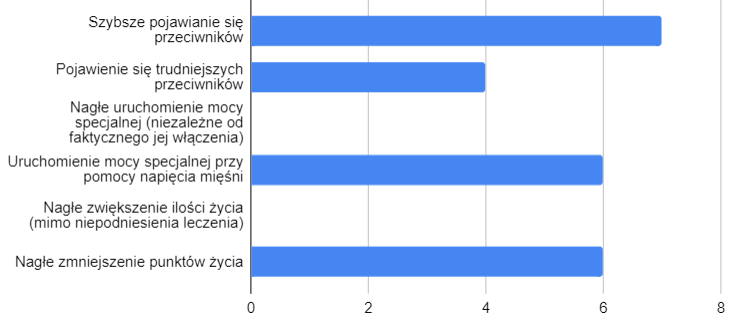
\includegraphics[width=0.8\linewidth]{images/affective_mechanics_seen.png}
	\caption{Zauważenie mechanik afektywnych przez uczestników badań}
	\label{fig:seen_mechanics}
\end{figure}

Ponieważ część mechanik afektywnych pokrywała się z~elementami rozgrywki w~wersji podstawowej, badane osoby zostały zapytane o~to, którą wersję mechaniki preferują (tab.~\ref{tab:prefered_mechanics}). W~przypadku uruchomienia mocy specjalnej i~aktywacji trybu trudnego gry, sześć osób zgodnie wybrała wersję afektywną. Opinie jednak były podzielone w~przypadku mechaniki kontroli punktów życia, gdzie połowa osób wybrała wersję podstawową. Wybór ten mógł być spowodowany przede wszystkim źle zaprojektowanymi mechanikami afektywnymi, które w~przypadku zrelaksowania karały gracza poprzez odebranie mu punktów życia. Jedna z~badanych osób nie zauważyła różnicy w~przypadku dwóch mechanik, natomiast wybrała wersję podstawową uruchamiania mocy specjalnej. Taki wybór mógł wyniknąć z~powodu wadliwości elektrod, które w~trakcie odczytów z~elektromiografu mogły zostać naruszone, przez co średnia wartość nie była na tyle wysoka, aby aktywować mechanikę.
\begin{table}[]
	\centering
	\caption{Wybór preferowanej wersji mechanik zaimplementowanych w~obu wersjach gry}
	\label{tab:prefered_mechanics}
	\begin{tabular}{|l|c|c|c|}
		\hline
		& \textbf{\begin{tabular}[c]{@{}c@{}}wersja \\ podstawowa\end{tabular}} & \textbf{\begin{tabular}[c]{@{}c@{}}wersja z~pętlą\\ afektywną\end{tabular}} & \textbf{Bez różnicy} \\ \hline
		\textbf{Uruchomienie mocy specjalnej} & 1~& 6~& 0~\\ \hline
		\textbf{\begin{tabular}[c]{@{}l@{}}Pojawianie się trudniejszych \\ przeciwników (tryb trudny)\end{tabular}} & 0~& 6~& 1~\\ \hline
		\textbf{Kontrola punktów życia} & 3~& 3~& 1~\\ \hline
	\end{tabular}
\end{table}

W ramach dodatkowych uwag badane osoby głównie zwróciły uwagę na pomiar przy pomocy elektrod, który określiły jako mało inwazyjny. Jedna osoba opisała gry wykorzystujące pętlę afektywną jako ciekawe nowe wyzwanie, które wymaga skupienia się nie tylko na rozgrywce, ale również na swoich emocjach i~reakcjach. Podczas rozmów badane osoby wskazywały elementy, które można poprawić w~grze, takie jak wspomniane wcześniej mechaniki afektywne. 

